\section*{Введение}
\addcontentsline{toc}{section}{Введение}

\TeX~--- система компьютерной вёрстки, разработанная американским профессором информатики Дональдом Кнутом в целях создания компьютерной типографии.  В неё входят средства для секционирования документов, для работы с перекрёстными ссылками и др. Многие считают \TeX~лучшим способом для набора сложных математических формул. В частности, благодаря этим возможностям, \TeX~популярен в академических кругах, особенно среди математиков и физиков \cite{wiki:tex}.

Название произносится как ``тех'' (от греч. $\boldsymbol{\tau\varepsilon\chi\nu\eta}$ --- ``искусство'', ``мастерство''). В написании буква E опущена ниже T и X. \TeX~является свободным ПО. Для создания шрифтов совместно с \TeX’ом используется специально разработанная Д. Кнутом система METAFONT, в которой шрифты описываются программами на специализированном языке Meta \cite{wiki:tex}.

\LaTeX~--- система верстки, ориентированная на производство научных математических документов высокого типографского качества \cite{introlatex}. По сути, \LaTeX~является средством автоматизации верстки документов при помощи \TeX. И если, набирая текст в WYSIWYG-редакторе, далее следует фаза настройки стилей, выравнивания и прочей утомительной верстки, то \LaTeX~позволяет не зацикливаться на самой верстке, а углубиться в написание и структурирование материала. К тому же, качество получившегося документа в разы превосходит качество, с которыми имеют дело текстовые процессоры (рисунок \ref{fig:quality}, сверху --- \LaTeX).

\begin{figure}[ht]
    
\includegraphics[width=.2\linewidth]{Figures/quality.png}
    \caption{Сравнение WYSIWYG и \LaTeX}
    \label{fig:quality}
\end{figure}

\section{История создания}

История создания этой типографической системы начинается в далеком 1962, когда Дональд Кнут начал писать свою известную книгу ``Искусство программирования'' (The Art of Computer Programming). В 1969 году был опубликован первый том книги и печатался методом монотипии, технологии XIX века, которая давала на выходе издание в ``хорошем классическом стиле'', что нравилось Кнуту. Когда в 1976 году публиковалось второе издание второго тома, всю книгу пришлось набирать вновь, поскольку монотипия почти повсеместно была замещена фотографической техникой, и оригинальные шрифты больше не использовались. Однако 30 марта 1977 года, когда Кнут получил новые оттиски, он увидел, что они выглядят ужасно. Примерно в это же время Кнут впервые увидел результат работы высококачественной цифровой типографической системы и заинтересовался возможностями цифровой типографии. Не оправдавшие ожиданий оттиски дали ему дополнительный толчок к тому, чтобы, разработав свою типографическую систему, решить проблему раз и навсегда. 13 мая 1977 года он написал заметку самому себе, описывающую базовые возможности \TeX’а.

С версии 3.0 \TeX~использует оригинальную систему нумерации версий: каждое обновление добавляет дополнительную десятичную цифру в конце номера версии так, что она асимптотически приближается к $\pi$. Это отражает тот факт, что текущая версия \TeX’а --- 3.1415926 --- очень стабильна и возможны лишь мелкие обновления. Последнее обновление было в марте 2008 года. На версии 3.0 дизайн системы был заморожен, поэтому добавление новой функциональности не планируется и все новые версии будут содержать только исправления ошибок. Хотя Дональд Кнут сам предложил несколько областей, в которых \TeX~мог бы быть улучшен, он тем не менее считал, что существование неизменной версии, которая бы выдавала одинаковый результат сейчас и в будущем, важнее, чем добавление новых возможностей. Поэтому он заявил, что ``совершенно последнее изменение (сделанное после моей смерти)'' сменит номер версии на $\pi$, и с этого момента ``все баги станут фичами''. Точно так же версии системы METAFONT начиная с версии 2.0 асимптотически приближаются к $e$ и так же завершатся на $e$ после смерти Кнута.

Ядро \TeX’а представляет собой язык низкоуровневой разметки, содержащий команды отступа и смены шрифта. Огромные возможности в \TeX’е предоставляют готовые наборы макросов и расширений. Наиболее распространённые расширения стандартного \TeX’а (наборы шаблонов, стилей и т. д): \LaTeX, произносится ``латех'' или ``лейтех'', и AMS-\TeX. При использовании пакета расширения \LaTeX~можно превратить разросшуюся статью в книгу изменением одного слова в исходнике, вставлять оглавление одной командой, не задумываться о нумерации разделов, теорем, рисунков. Есть много пакетов для оформления химических формул (например, пакет Xym\TeX), диаграмм (xypic), создания презентаций (beamer), визитных карточек и тому подобного. Все это распространяется путем внешних пакетов на CTAN --- Comprehensive \TeX Archive Network. На сегодняшний день (25 октября 2014 г.) на CTAN насчитывается 4783 пакета, поддерживаемые 2225-ю авторами. Достаточно зайти на \url{http://www.ctan.org/}, найти нужный пакет, прочитать документацию, скачать и начать использовать. Существует множество интересных пакетов, как для красивой верстки, так и для верстки разнообразных формул (рисунок \ref{fig:example}). Более подробно о внешних пакетах \LaTeX~будет рассказано в главе \ref{sec:ext} (\nameref{sec:ext}).

\begin{figure}[ht]
    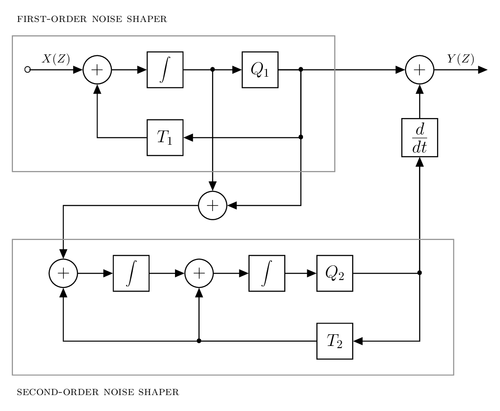
\includegraphics[width=.6\linewidth]{Figures/example.png}
    \caption{Пример схемы на \LaTeX~используя tikz}
    \label{fig:example}
\end{figure}

\section{Сравнение \LaTeX~и текстовых процессоров} %Зачем это нужно

У человека, привыкшего к тектовым процессорам WYSIWYG (What You See Is What You Get, что видишь --- то и получаешь) может возникнуть справедливый вопрос: а зачем мне это надо? Предположим, нас не интересует качество результата, нам не нужно набирать формул. Мы формируем небольшой документ, гуманитарный реферат или письмо другу. В данной ситуации, конечно, \LaTeX~использовать нужды нет.

А теперь, предположим, нам нужно набрать диссертацию с кучей формул, таблиц, графиков и схем, да еще все по ГОСТу. Набирать такой документ в текстовом процессоре, который для этого совершенно не предназначен --- сущее извращение. В такой ситуации будет полезно воспользоваться \LaTeX-ом.

График, отражающий зависимость необходимых усилий для создания документа от сложности документа представлен на рисунке \ref{fig:graph}.

\begin{figure}[ht]
    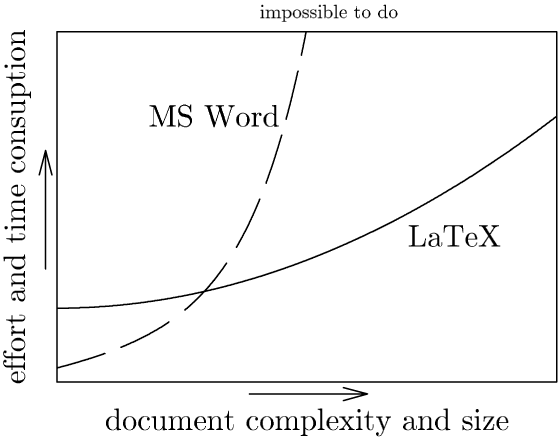
\includegraphics[width=.6\linewidth]{Figures/graph.png}
    \caption{Зависимость усилий от сложности документа}
    \label{fig:graph}
\end{figure}

Перечислим плюсы \LaTeX:

\begin{itemize}
    \item качество выходного документа;
    \item бесплатность и открытость;
    \item удобство (нумерация, содержание, набор формул);
    \item концентрация на содержимом;
    \item возможность коллективной работы;
    \item переносимость;
    \item программируемые графики и схемы.
\end{itemize}

Основное преимущество \LaTeX~перед текстовыми процессорами --- это несомненно высокое типографическое качество документа. Для примера, рассмотрим разницу строки текста в MS Word и \LaTeX~(рисунок \ref{fig:difference}, \LaTeX --- сверху).

\begin{figure}[ht]
    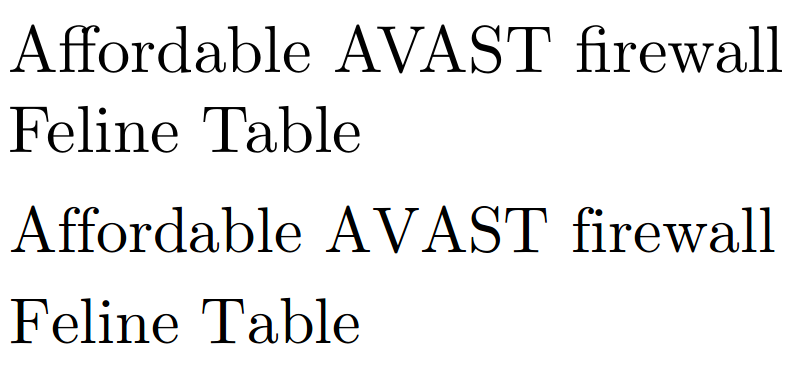
\includegraphics[width=.6\linewidth]{Figures/difference.png}
    \caption{Разница MS Word и \LaTeX}
    \label{fig:difference}
\end{figure}

На первый взгляд, может показаться что разницы нет. Однако, присмотревшись, можно заметить что в MS Word нет связок ``ff'' и ``fi'', неправильное расстояние между ``Fe'' и ``Ta'', а в ``AVA'' вообще ужасно. В больших текстах такие мелочи придают всему тексту ужасный вид, незаметный для привыкших пользователей текстовых процессоров.

Удобство \LaTeX~в плане набора формул просто поражает. Формулы можно набирать прямо как текст. Например, код

\begin{minted}[breaklines,gobble=4,fontsize=\small]{latex}
    \sum\limits_{k=1}^{\sigma} f_k(x,u) = \int\limits_a^x \frac{dx}{\sqrt{x^2 + a^2}}
\end{minted}

произведет формулу $\sum\limits_{k=1}^{\sigma} f_k(x,u) = \int\limits_a^x \frac{dx}{\sqrt{x^2 + a^2}}$.

Также \LaTeX~занимается автоматической нумерацией рисунков, таблиц, формул, созданием содержимого и всем остальным, пользователю не нужно задумываться об этом. Позволяя четко разделить форматирование документа и контент, \LaTeX~предоставляет возможность сконцентрироваться на содержимом документа и его структуре, т.е. думать о том, что будет содержать документ, а не о том, как он будет выглядеть на бумаге, в то время как в текстовых процессорах постоянно необходимо думать о стилях, выравниваниях и съезжающих строках.

Возможна коллективная работа над документом \LaTeX. Если разбить документ на несколько файлов, а в главном документе прописать подключение этих файлов последовательно их расположению, можно раздать эти файлы разным участникам проекта и каждый будет трудиться над своей частью. Тем временем, коллективная работа будет кипеть над всем документом.

Стоит сказать пару слов и о переносимости. Из-за черезвычайной стабильности \TeX, документы, созданные 10 лет назад, скомпилируются без проблем и сейчас и будут выглядеть одинаково, скомпилированные на любой машине под любой операционной системой.

И последний плюс, перечисленный здесь, хотя их несомненно гораздо больше: программируемые графики и схемы. Предположим, нам нужно вставить в документ большую сложную схему или график. Рисуя схему во внешнем ПО, вы вставляете готовое изображение в документ. Однако, если что-то нарисовано неправильно, придется загружать внешнее ПО и менять картинку, что может быть достаточно трудоемкой задачей. Если же вы нарисовали данную схему используя \LaTeX, все что нужно --- это поменять пару переменных и перекомпилировать документ. Картинка автоматически изменится под ваши нужды.

Существует множество пакетов для рисования блок-схем, графов, электрических принципиальных и логических схем, контуров САУ, чертежей и т.п. Пример изображен на рисунке \ref{fig:example}. Подробнее об этих экзотических пакетах будет рассмотрено в главе \ref{sec:exotic} (\nameref{sec:exotic}).

Пара слов о том, когда не нужно использовать \LaTeX:

\begin{itemize}
    \item когда нет времени его учить (например, если нужно составить документ за 24 часа, а знаний \LaTeX~у вас нет);
    \item если документ уже написан в текстовом процессоре (незачем тратить время на перепись, если только вас не интересует качество печати);
    \item если необходим креативный дизайн (\LaTeX~--- набор правил, а не система дизайна; для дизайна сложных журналов и постеров лучше использовать специализированные пакеты вроде scribus).
\end{itemize}

\section{Обзор макропакета \LaTeX}

\LaTeX~--- наиболее популярный набор макрорасширений (или макропакет) системы компьютерной вёрстки \TeX, который облегчает набор сложных документов \cite{wiki:latex}.

Первая версия была выпущена Лесли Лэмпортом в 1984 году; текущая версия, после создания в 1994 году испытывала некоторый период нестабильности, окончившийся к концу 90-х годов, а в настоящее время стабилизировалась (хотя раз в год выходит новая версия).

Общий внешний вид документа в LaTeX определяется стилевым файлом. Существует несколько стандартных стилевых файлов для статей, книг, писем и т. д., кроме того, многие издательства и журналы предоставляют свои собственные стилевые файлы, что позволяет быстро оформить публикацию, соответствующую стандартам издания.

Во многих развитых компьютерных аналитических системах, например, Maple, Mathematica, Maxima, Reduce возможен экспорт документов в формат *.tex. Для представления формул в Википедии также используется \TeX-нотация.

Термин \LaTeX~относится только к языку разметки, он не является текстовым редактором. Для того, чтобы создать документ с его помощью, надо набрать .tex-файл с помощью какого-нибудь текстового редактора. В принципе, подойдёт любой редактор, но большая часть людей предпочитает использовать специализированные, которые так или иначе облегчают работу по набору текста \LaTeX-разметки.

Главная идея \LaTeX~состоит в том, что авторы должны думать о содержании, о том, что они пишут, не беспокоясь о конечном визуальном облике (печатный вариант, текст на экране монитора или что-то другое). Готовя свой документ, автор указывает логическую структуру текста (разбивая его на главы, разделы, таблицы, изображения), а \LaTeX~решает вопросы его отображения. Так содержание отделяется от оформления. Оформление при этом или определяется заранее (стандартное), или разрабатывается для конкретного документа.

\subsection{Возможности \LaTeX}

\LaTeX~расширяет возможности голого \TeX, автоматизируя многие вещи при помощи макросов и внешних пакетов, содержащих свои макросы. Для примера, стандартный блок нумерованного списка выглядит так:

\begin{minted}[gobble=4,fontsize=\small]{latex}
    \begin{enumerate}
        \item Первый пункт.
        \item Второй пункт.
    \end{enumerate}
\end{minted}

Этот функционал предоставляется пакетом \textbf{enumerate}, так что при использовании в чистом \TeX~вам пришлось бы написать

\mint[fontsize=\small]{latex}|\usepackage{enumerate}|

Эта команда подключает внешний пакет. Но в \LaTeX~этот пакет подключен по умолчанию, так что структуры \textbf{enumerate} можно использовать из коробки.

Если бы мы захотели описать нумерованный список на чистом \TeX, не используя пакет \textbf{enumerate}, нам бы пришлось написать кучу кода по выравниванию символов и позиционированию элементов, т.е. другими словами --- написать этот самый пакет \textbf{enumerate}.

\LaTeX~и \TeX~можно сравнить с C и assembler. Первый --- мощный автоматизированный инструмент, использующий assembler (\TeX) для компиляции своих структур, второй --- непосредственно сама система типографии, осуществляющая низкоуровневое позиционирования шрифтов и элементов документа.

Возможности \LaTeX:

\begin{itemize}
    \item алгоритмы расстановки переносов, определения междусловных пробелов, балансировки текста в абзацах;
    \item автоматическая генерация содержания, списка иллюстраций, таблиц и т. д.;
    \item механизм работы с перекрёстными ссылками на формулы, таблицы, иллюстрации, их номер или страницу;
    \item механизм цитирования библиографических источников, работы с библиографическими картотеками;
    \item размещение иллюстраций (иллюстрации, таблицы и подписи к ним автоматически размещаются на странице и нумеруются);
    \item оформление математических формул, возможность набирать многострочные формулы, большой выбор математических символов;
    \item оформление химических формул и структурных схем молекул органической и неорганической химии;
    \item оформление графов, схем, диаграмм, синтаксических графов;
    \item оформление алгоритмов, исходных текстов программ (которые могут включаться в текст непосредственно из своих файлов) с синтаксической подсветкой;
    \item разбивка документа на отдельные части (тематические карты).
\end{itemize}

Расширенные средства работы с библиографическими данными предоставляются программой Bib\TeX. Базовые возможности работы с математическими формулами расширяются с помощью пакета AMS-\LaTeX.

\subsection{Примеры использования}

Вставка рисунка в \LaTeX~осуществляется следующим образом:

\begin{minted}[breaklines,gobble=4,fontsize=\small]{latex}
    Ссылка на картинку --- рисунок \ref{fig:somepicture}.

    \begin{figure}[ht]
        \subcaptionbox{}{
            $\alpha = \left| \begin{matrix}
                1 & 0 & 0\\
                0 & 1 & 1\\
                0 & 0 & 1
            \end{matrix} \right|.$
        }
        \qquad
        \subcaptionbox{}{
            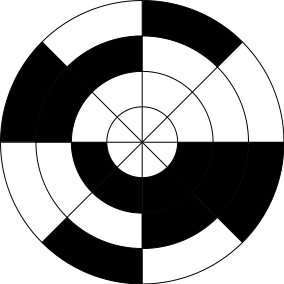
\includegraphics[width=.2\linewidth] {Figures/somepicture.png}
        }
        \caption{Пример рисунка (а) матрица, описанная при помощи \LaTeX; (б) картинка}
        \label{fig:somepicture}
    \end{figure}
\end{minted}

В результате получим следующее:

Ссылка на картинку --- рисунок \ref{fig:somepicture}.

\begin{figure}[ht]
    \subcaptionbox{}{
        $\alpha = \left| \begin{matrix}
            1 & 0 & 0\\
            0 & 1 & 1\\
            0 & 0 & 1
        \end{matrix} \right|.$
    }
    \qquad
    \subcaptionbox{}{
        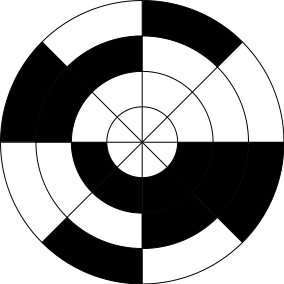
\includegraphics[width=.2\linewidth]{Figures/somepicture.png}
    }
    \caption{Пример рисунка (а) матрица, описанная при помощи \LaTeX; (б) картинка}
    \label{fig:somepicture}
\end{figure}

Для таблиц и листингов используется схожая конструкция. Для автоматической нумерации формул можно использовать конструкцию

\begin{minted}[gobble=4,fontsize=\small]{latex}
    Ссылка на формулу --- формула \ref{eq:some}.

    \begin{equation}
        \int\limits_0^\pi x dx = \textup{\Huge{?}}
        \label{eq:some}
    \end{equation}
\end{minted}

Получим:

Ссылка на формулу --- формула \ref{eq:some}.

\begin{equation}
    \int\limits_0^\pi x dx = \textup{\Huge{?}}
    \label{eq:some}
\end{equation}

\section{Структура документа}

Документ \LaTeX~--- это текстовый файл, содержащий специальные команды языка разметки. Сам документ делится на преамбулу и тело. Преамбула содержит информацию про класс документа, использованные пакеты макросов, определения макросов, автора, дату создания документа и другую информацию. Тело документа содержит собственно текст документа и команды разметки.

Любой документ начинается с указания используемого класса:

\begin{minted}[gobble=4,fontsize=\small]{latex}
    \documentclass{article}
\end{minted}

Существуют классы article, report, book и другие, а также множество пакетов расширений и других классов. Например, класс \textbf{article} содержит параметры только для шрифтов 10pt, 11pt и 12pt. Для того, чтобы добиться шрифта 14pt, используемого в курсовых и дипломных работах, необходимо использовать внешний класс \textbf{extarticle}. В данном документе, например, первая строка преамбулы выглядит так:

\inputminted[breaklines,firstline=1,lastline=1,fontsize=\small]{latex}{../preamble.tex}

Как видно из кода, здесь также используется параметр \textbf{a4paper}, который отвечает за установку размера листа. Он необходим т.к. по умолчанию в \LaTeX~используется стандартный американский размер бумаги \textbf{US letter}. Он на 18 мм короче и на 8 мм шире по сравнению с мировым А4 форматом.

Далее указываются остальные директивы преамбулы, отвечающие за уникальную верстку всего документа. Например, описать полностью ГОСТ оформления дипломной работы можно всего в 150 -- 200 строк кода преамбулы. После преамбулы идет тело документа, заключенное командами:

\begin{minted}[gobble=4,fontsize=\small]{latex}
    \begin{document}
    %Здесь располагается тело документа
    \end{document}
\end{minted}

Как можно предположить исходя из кода, комментарии в \TeX~начинаются со знака процента. В теле располагется весь основной текст документа, отформатированный средствами \TeX~и \LaTeX.

Также для большей гибкости документ можно разбивать на несколько файлов. Например, тело документа написать в файле \textbf{body.tex}, преамбулу --- в документе \textbf{preamble.tex}, титульный лист --- в файле \textbf{title.tex}, а главный компилируемый файл, который будет включать все остальные файлы, назовем \textbf{main.tex}. Его содержимое:

\inputminted[fontsize=\small]{latex}{main.tex}

Также для удобства можно разложить отдельные разделы документа по своим файлам.

Команда \textbf{input}, как следует из ее названия, вставляет кусок кода из другого файла. Соответственно, преамбулу вставляем в самом начале. Две точки и слеш перед файлом в системах семейства \textbf{UNIX} означают переход в директорию на уровень выше. Это означает, что файл \textbf{preamble.tex} лежит на один уровень выше текущей папки. Сделано это для того, чтобы использовать одну преамбулу на все документы, разложенные по разным папкам в одной общей папке с файлом преамбулы. Расширения файлов не указаны, т.к. компилятор \textbf{pdflatex} автоматически приписывает \textbf{.tex} расширение к именам в директиве \textbf{include}. Команда \textbf{tableofcontents} между титульной страницей и остальным телом --- это специальная директива, которая на основании всего текста документа автоматически формирует содержание по всем правилам, указанным в преамбуле.

Для структурирования тела документа используются команды типа \textbf{section}, \textbf{subsection}, \textbf{subsubsection} и т.п., например

\mint[fontsize=\small]{latex}|\section{Основные команды \TeX}|

Все идущее после такой команды будет автоматически включено в этот раздел (идти после названия раздела), а команда \textbf{tableofcontents}, генерирующая содержание, автоматически включит и пронумерует все разделы и подразделы.

Для создания разделов без нумерации, достаточно поставить знак звездочки после команды, например

\mint[fontsize=\small]{latex}|\section*{Введение}|

Вернемся к началу преамбулы. Для того, чтобы \LaTeX~мог читать кириллические символы в кодировке \textbf{utf-8}, необходимо проделать ряд телодвижений. Начало преамбулы данного документа представлено ниже:

\inputminted[breaklines,firstline=1,lastline=6,fontsize=\small]{latex}{../preamble.tex}

Здесь во второй строке подключается пакет \textbf{cmap}, отвечающий за то, что при копировании наших символов из PDF-файла мы не получим крякозябров, а получим вполне адекватный кириллический текст.

Далее подключается пакет \textbf{fontenc}, подключающий таблицу кириллических символов T2A. Пакет \textbf{inputenc}, в свою очередь, устанавливает кодировку входных и выходных файлов в utf-8, поддерживаемую таблицей T2A.

Пакет \textbf{babel} отвечает за семантический анализ текста, переносы и перевод стандартных названий элементов \LaTeX. Здесь указан английский язык, чтобы не потерять английские переносы. Русский язык указан последним, чтобы элементы \LaTeX~перевелись на русский язык (например, ``chapter'' будет переведена как ``глава'', а ``table of contents'' --- как ``содержание'').

Последний пакет --- \textbf{pscyr}, содержит профессиональные каллиграфические кириллические шрифты, еще более качественные чем в стандартном пакете.

\section{Основные команды \TeX}

Существует ряд основных правил и команд \TeX, которые не поддаются автоматизации \LaTeX. Составляя документ в данной системе верстки пользователь непосредственно будет иметь дело с этими командами. В этой главе будет дан краткий обзор основных возможностей \TeX и его команд.

Для изменение шрифта или атрибутов текста (жирный, курсив) используются т.н. теги: \textbf{textbf}, \textit{textit}, \textrm{textrm} и т.п.

Формулы заключаются между знаками доллара или в среду \textbf{equation} если формула большая и нам требуется нумерация (функция \LaTeX).

Также существует три типа тире:

\begin{itemize}
    \item - (-) обычное тире, минус;
    \item - - (--) среднее тире, для обозначения диапазона (страниц, например);
    \item - - - (---) длинное тире, для прямой речи и объяснений.
\end{itemize}

Кавычки --- отдельный разговор. Для того, чтобы произвести кавычки ``такого вида'' необходимо отдельно указать две открывающие, а потом две закрывающие кавычки. Выглядит это вот так:

\mint[fontsize=\small]{latex}|``Двойные кавычки'', `Одинарные кавычки', А'построф.|

``Двойные кавычки'', `Одинарные кавычки', А'построф.

Для принудительного перехода на новую строку применяется двойной обратный слеш, для начала новой страницы --- команда \textbf{newpage} и т.д. В принципе, верстка документа сложностей не вызывает, на деле это оказывается даже проще \textbf{html}.

\section{Наиболее популярные пакеты \LaTeX}
\label{sec:ext}

\subsection{Стандартные пакеты настройки содержимого}

Разберем основные пакеты для настройки верстки, использованные в этом документе.

\inputminted[breaklines,firstline=8,lastline=15,fontsize=\small]{latex}{../preamble.tex}

Здесь пакет \textbf{graphicx} отвечает за вставку изображений. Пакет \textbf{caption} позволяет изменить стандартную надпись ``Рис.'' на ``Рисунок'', соответствующую нашему ГОСТу. Параметр этого пакета \textbf{justification=centering} указывает на то, что по умолчанию все названия рисунков, таблиц и прочих плавающих объектов будут размещены по центру.

Далее следует настройка, собственно, надписи ``Рисунок'', разделителя в виде длинного тире, а последняя строка указывает, что счетчик рисунков должен соответствовать разделу, в котором рисунок находится (например, 1.1). По умолчанию рисунки имеют сквозную нумерацию (рисунок 1, 2, 3).

\inputminted[breaklines,firstline=17,lastline=21,fontsize=\small]{latex}{../preamble.tex}

Пакет \textbf{indentfirst} устанавливает автоматические абзацы первого параграфа с красной строки. Далее устанавливается междустрочный интервал, шрифт Times New Roman и \textbf{frenchspacing} --- команда, устанавливающая количество пробелом между словами равным 1 (по умолчанию, их 2).

\inputminted[breaklines,firstline=23,lastline=27,fontsize=\small]{latex}{../preamble.tex}

Пакет \textbf{geometry} отвечает за установку отступов от краев листа.

Можно еще долго перечислять полезные пакеты \LaTeX, но это основные, участвующие в первоначальном формировании документа.

\subsection{Экзотические пакеты}
\label{sec:exotic}

Существует много интересных пакетов \LaTeX, позволяющих оформлять графики, карты Карно, схемы и т.п., например --- \textbf{tikz}.

\mint[fontsize=\small]{latex}|\usepackage{tikz}|

С помощью нее можно рисовать как евклидову геометрию, так и электрические принципиальные схемы. От блок-схем систем автоматического управления до схем на логических элементах. И синтаксис достаточно понятен и логичен.

Примеры схем, выполненных при помощи пакета tikz, показаны на рисунке \ref{fig:tikzex}.

\begin{figure}[!ht]
    \subcaptionbox{}{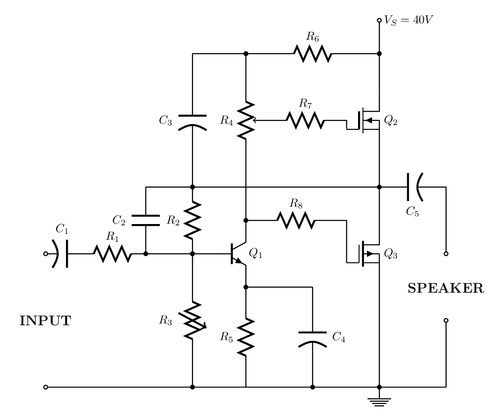
\includegraphics[width=.4\linewidth]{Figures/ex1.png}}
    \subcaptionbox{}{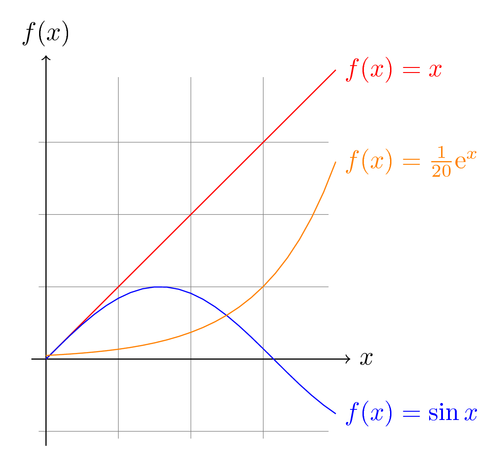
\includegraphics[width=.4\linewidth]{Figures/ex3.png}}

    \subcaptionbox{}{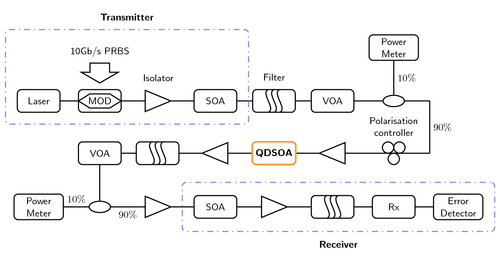
\includegraphics[width=.7\linewidth]{Figures/ex2.png}}
    \caption{Примеры tikz (а) электрическая принципиальная схема; (б) график; (в) блок-схема}
    \label{fig:tikzex}
\end{figure}

Также существует пакет \textbf{beamer}, отвечающий за создание презентаций. Да, при помощи \LaTeX~можно создать PDF-презентации и показывать их средствами PDF-просмотрщика, поддерживающего режим презентаций, например Impressive .Подробнее об этом в разделах \ref{sec:beamer} (\nameref{sec:beamer}).

Помимо всех этих пакетов для верстки документов, существуют пакеты с предопределенными правилами. Например, пакет \textbf{dissert}. Этот пакет включает набор правил, основанных на ГОСТах, и предназначен для написания диссертаций и дипломных работ. То есть взяв этот пакет, не надо будет составлять преамбулу вручную, достаточно будет подключить dissert к документу и документ сверстается по всем ГОСТам. Однако все-же гораздо более практично разобраться в преамбуле самому и настроить всё до мельчайших деталей, зная где что используется, а не включив пакет с кучей неизвестных правил, т.к. во втором случае можно ждать чего угодно.

\subsection{BiB\TeX~--- система оформления библиографических источников}

В \LaTeX есть встроенная возможность указывать библиографические источники следующим образом:

\begin{minted}[gobble=4,fontsize=\small]{latex}
    \begin{thebibliography}{9}
        \bibitem{lamport94}
            Leslie Lamport,
            \emph{\LaTeX: a document preparation system}.
            Addison Wesley, Massachusetts,
            2nd edition,
            1994.
    \end{thebibliography}
\end{minted}

Таким манером указываются все источники под конец документа, а в самом документе ссылаются на них, используя конструкцию

\mint[fontsize=\small]{latex}|\cite{lamport94}|

Однако в такой системе существует ряд недостатков:

\begin{enumerate}
    \item Источники указываются в порядке их указания в списке источников, т.е. если вам вдруг вздумается поменять местами два абзаца с разными цитируемыми источниками, то в результате сначала будет цитироваться [2], и только потом --- [1].
    \item Среда \textbf{thebibliography} не знает, что есть что, а просто выдает источник в том виде, в котором он указан, соответственно нельзя отредактировать стиль источника, соответствующий нашему ГОСТу.
    \item Эти источники нельзя будет использовать в другом документе --- система не является гибкой.
\end{enumerate}

Существует мощная альтернатива --- система библиографических ссылок BiB\TeX. При её использовании, вся литература хранится в одной отдельной базе данных, и в теле документа достаточно указать

\mint[fontsize=\small]{latex}|\bibliography{../web}|

Здесь указывается файл \textbf{web.bib}, который лежит на одну директорию выше текущей (также, как и \textbf{preamble.tex}) и имеет много пунктов следующего содержания:

\inputminted[breaklines,firstline=3,lastline=7,fontsize=\small]{latex}{../web.bib}

В итоге, база данных хранит всю литературу, найденную за все время, а все документы подключают одну и ту же базу (как и в случае с преамбулой).

Помимо такого удобства, BiB\TeX автоматически подключит только ту литературу, на которую ссылались в тексте, отформатирует ее в формате, заданном в преамбуле, и упорядочит ее в порядке цитирования в тексте.

\section{Редактирование и компиляция}

\subsection{Редакторы \LaTeX}

Для редактирования \LaTeX-кода можно пользоваться хоть блокнотом, но люди предпочитают пользоваться т.н. IDE --- программами с подсветкой синтаксиса и прочими помощниками. Я, как заядлый пользователь \textbf{VIM}, пользуюсь им для создания \LaTeX-документов, используя также плагин \textbf{snipmates} и собственноручно созданные сниппеты для него. Для обычного пользователя будет больше удобна IDE.

Среди хороших \LaTeX-IDE нельзя не отметить \TeX studio. Это кроссплатформенная среда разработки на \LaTeX, имеющая богатые возможности подсветки кода, управление библиографией, автоматической установкой необходимых пакетов и удобным PDF-просмотрщиком готовых результатов. Она включает множество инструментов для облегчения работы начинающим пользователям.

Используя IDE, у вас будет возможность безболезненно компилировать и просматривать код. Но если вы все-же используете консоль, вим и стандартные утилиты компиляции латека (как latex и pdflatex), будет полезно знать некоторые хитрости компиляции.

\subsection{Изъяны компиляции}

Для правильной компиляции перекрестных ссылок, названий таблиц и рисунков, необходимо производить компиляцию дважды подряд. Первый раз формируется сам документ, рисунки и таблицы, но т.к. ссылки на эти рисунки указываются перед, непосредственно, рисунками --- они не могут найти рисунка и интерпретируются как пустые (знаками вопроса). При второй же компиляции, ссылки на объекты формируются правильным образом.

При использовании пакета BiB\TeX, необходимо отдельно компилировать библиографию. Делается это следующим образом: сначала компилируется документ один раз, затем один раз --- библиография, и потом еще два раза компилируется сам документ. Например:

\begin{minted}[gobble=4,fontsize=\small]{latex}
    pdflatex main
    bibtex main
    pdflatex main
    pdflatex main
\end{minted}

Для таких целей будет разумно написать автоматизированный скрипт, который будет выполнять всю эту работу и, также, перемещать готовый pdf-файл куда вам необходимо. Пример такого скрипта приведен в приложении A.

\subsection{Альтернатива \LaTeX~--- Xe\TeX}

У \TeX~существует немного конкурентов в сфере типографической верстки документов, но существует много разных пакетов, схожих с \LaTeX, основывающихся на \TeX~и предоставляющих похожие возможности. Один из таких пакетов --- Xe\TeX.

Главное преимущество Xe\TeX-а в том, что он поддерживает юникод, т.е. символы кодировки utf-8 можно писать прямо в теле документа, не используя изощренные математические режимы и контрольные слова.

У пользователей \LaTeX~время от времени возникают проблемы с utf-8-кодировкой. Иногда это несовместимость с пакетами, иногда --- невозможность указать некоторые символы как слова. Факт в том, что \LaTeX~еще не до конца поддерживает юникод, а я --- большой фанат юникода. Как альтернатива, рассматривается Xe\TeX.

Xe\TeX~был создан в 2004 году Джонатаном Кью как очередная модификация над движком с целью поддержки широкой области символов за пределами чистого английского (ASCII) и поддержки современных форматов шрифтов. В результате получился пакет, похожий на \LaTeX~по функциональности, но более удобный для не англоязычных пользователей (с родной поддержкой юникода). Поэтому Xe\TeX~может рассматриваться как более подходящий инструмент, на который стоит перейти после \LaTeX~(вероятнее, на Xe\LaTeX).

\section{Создание презентаций средствами \LaTeX}
\label{sec:beamer}

\subsection{Обзор пакета beamer}

Пакет \textbf{beamer} позволяет создать PDF-презентацию средствами \LaTeX, beamer является классом документа, устанавливающим соответствующие правила и размеры слайда 4:3. Первая строка преамбулы, в данном случае, будет выглядеть так:

\inputminted[breaklines,firstline=3,lastline=3,fontsize=\small]{latex}{/home/ewancoder/Dropbox/LaRep/beamer.tex}

Каждый слайд заключается в среду \textbf{frame}:

\begin{minted}[gobble=4,fontsize=\small]{latex}
    \begin{frame}
        Slide content
    \end{frame}
\end{minted}

Если необходимо задать динамику (например, появляющиеся один за одним элементы списка), это можно сделать командой \textbf{pause}:

\begin{minted}[gobble=4,fontsize=\small]{latex}
    \begin{frame}
        \begin{itemize}
            \pause\item Первый пункт;
            \pause\item Второй пункт;
            \pause\item Третий пункт.
        \end{itemize}
    \end{frame}
\end{minted}

В результате будут созданы 4 слайда вместо одного, на первом не будет ни одного элемента списка, на втором --- будет лишь первый элемент, на третьем --- два первых и на последнем --- все. При просмотре PDF в режиме презентации, при переключении между этими слайдами будет создаваться видимость появления элементов списка.

\subsection{Обзор PDF-просмотрщика Impressive}

PDF-просмотрщик Impressive предназначен специально для воспроизведения PDF-презентаций с красивыми эффектными переходами. Impressive написан на python с использованием xpdf для PDF-рендеринга и OpenGL в связке с pygame для рендеринга окон. 

\clearpage
\section*{Заключение}
\addcontentsline{toc}{section}{Заключение}

\LaTeX~движется вперед по восходящей параболе оптимизма в светлое будущее, изменяя этот мир к лучшему. Можно с уверенностью сказать, что для больших технических текстов \LaTeX~несомненно является более предпочтительной системой нежели текстовые процессоры, набор формул в которых зачастую сложен, а набор схем зачастую и невозможен без стороннего ПО. Используя \LaTeX, можно сэкономить время на оформлении стилей, выравнивании текста и беспокойстве о внешнем виде документа, и потратить это время на, непосредственно, составление самого текста.

Дональд Кнут в свое время создал великую вещь, позволяющую нам сейчас, за счет существования CTAN, без проблем, автоматизированно и быстро создавать технические документы высокого типографического качества, а с учетом существования готовых ГОСТ-библиотек по типу \textbf{dissert}, можно и вовсе не задумываться о написании сложной преамбулы, а, подключив необходимый стиль, думать лишь о содержании.

\section*{Приложение А --- Скрипт компиляции}
\addcontentsline{toc}{section}{Приложение А --- Скрипт компиляции}

\inputminted[breaklines,fontsize=\small]{bash}{/home/ewancoder/bin/pl}

\clearpage
\bibliography{../web,../books}
